%Review of existing harmonic excitation.
%	Nonlinear Systems
%		Traditional Metrics (THD, IMD)
%		Minimisation of Nonlinear Distortion
%		Advent of "Nonlinear Niceness"
%	Timbre of nonlinear distortions (Martens and Marui type shit)
%	Uses of Harmonic Excitation
%	Harmonic Generation Methods
%		Static Nonlinearities
%		Bandwidth Extension (high frequency reconstruction)
%		Individual Harmonic Generation (SMC paper)
%		Psychoacoustic Enhancers

\addtocontents{toc}{\protect\newpage}
\chapter{Comparative Evaluation of Harmonic Excitation Algorithms}
\label{chap:ExcitationEvaluation}
	Harmonic excitation algorithms developed for the applications discussed in Section~\ref{sec:Excitation-Uses} are
	specialised to perform a particular task. As this work is concerned with the application of harmonic excitation to
	real time timbral control, some algorithms in the literature may not be suitable due to the predictability of their
	effects on a signal or their inability to operate in real time. In
	Section~\ref{sec:ExcitationEvaluation-Evaluation} a set of criteria for assessing the suitability of harmonic
	excitation algorithms for use in this work are suggested. These criteria are then used to asses various algorithms
	in Section~\ref{sec:ExcitationEvaluation-Comparison}, with a summary of each algorithm's performance shown in
	Table~\ref{tab:ComparisonSummary}. Techniques by which the performance of several algorithms can be improved, with
	respect to these criteria, are also discussed.

\section{Evaluating Harmonic Excitation Algorithms for Use in Timbral Control}
\label{sec:ExcitationEvaluation-Evaluation}
	To prove useful for real time timbral control, a harmonic excitation algorithm should provide efficient, intuitive
	control over where energy is introduced into a signal's spectrum. \citet{larsen2004audio} evaluate a number of
	algorithms for their use in bandwidth extension applications, discussing the spectral and temporal characteristics
	of the systems. Similar properties are required for algorithms used in real time timbral control, which will be
	assessed against the following criteria:

	\begin{itemize}
		\item Computational Complexity
		\item Homogeneity
		\item Spectral Characteristics
		\item Temporal Characteristics
		\item Use Cases
%		\item Naturalness.
	\end{itemize}

	Together, these criteria describe possible timbral manipulations an algorithm can be used for. The spectral and
	temporal characteristics describing the system's effects on low level features of a signal and complexity,
	homogeneity and use cases describing how well those can be utilised in a creative effect. Further detail on the
	ideal characteristics within these areas are discussed in Sections
	\ref{sec:ExcitationEvaluation-Evaluation-Complexity} to \ref{sec:ExcitationEvaluation-Evaluation-UseCases}.

	\subsection{Computational Complexity}
	\label{sec:ExcitationEvaluation-Evaluation-Complexity}
		Audio effects can operate either offline or in real time. An offline effect is provided with a prerecorded
		input signal and processes it, taking as much time as is necessary. A real time effect processes an input
		signal in a short enough time that the output can be produced at the same rate at which the input is being
		provided. Real time processing speeds up music production, as effect parameters can be adjusted while audio
		is playing and the results heard immediately. In order to achieve this, the algorithms used in the effect
		must be efficient and operate with minimal latency. 

		In order to ease the computational load on the processor, digital audio is often processed in blocks.  A
		certain number of samples are recorded into a memory buffer and then all processed at once. This introduces
		some latency into the system; the processing buffer must be filled with samples from the input before an
		output can be produced. The larger the processing buffer size the more latency but the less the
		computational load as the cost of constructing and moving buffers is amortised across a greater number of
		samples. Any processing applied to the block of audio must be completed within the latency time allowed by
		the buffer size, if not there will be gaps between blocks during playback, causing audible anomalies. For
		real time audio effects it is crucial to keep throughput latency to a minimum. \citet{lester2007the}
		suggest that, depending on the scenario, latencies as small as 1.4ms could be deemed unacceptable. In order
		to keep latency to a minimum, processing algorithms should be able to operate in real time when using a
		small buffer size.  Occasionally it is necessary to introduce a specific amount of delay as part of the
		processing algorithm, such as when applying a non-causal filter. This delay contributes to the overall
		latency of the effect and as such will be discussed alongside an algorithm's complexity.  In a modern music
		production setting there may be several audio effects operating concurrently, therefore the algorithms used
		for real time harmonic excitation must not only be efficient enough to run in real time, but also to allow
		any concurrent processing to proceed uninterrupted.

	\subsection{Homogeneity}
	\label{sec:ExcitationEvaluation-Evaluation-Homogeneity}
		To make the application of an audio effect more intuitive it should produce similar perceived timbral
		manipulations for all input signals. Often this is not the case with traditional audio signal processing
		methods. For example, an equaliser can be used to amplify a certain band of frequencies is a signal. This
		will have different effects depending on whether the input contains energy at these frequencies. The
		spectra of signals with energy in this frequency range will be altered, while those of signals with no
		energy in that band will be unaffected. This problem is compounded when the effect being applied is
		non-homogeneous (does not satisfy the condition of homogeneity given by Equation~\ref{eq:homogeneity}).
		Nonlinear systems are typically non-homogeneous; this is undesirable when using them to achieve timbral
		control as it means the effects are less easy to predict. A non-homogeneous system behaves differently
		depending on the amplitude of the input signal. Different timbral transforms could be applied to the same
		signal if its amplitude is changed slightly. From a user's point of view this makes control of the system
		less intuitive as the perceived function of control parameters can change depending on signal level. The
		algorithms used in harmonic excitation systems for timbral control should exhibit homogeneous behaviour in
		order to increase the system's intuitiveness.

		In the summary shown in Table~\ref{tab:ComparisonSummary} the homogeneity of the algorithms evaluated in
		this section is identified using four different terms. Homogeneous and non-homogeneous identify systems
		which do and do not satisfy the principle of homogeneity. Positive homogeneous refers to systems which are
		homogeneous for positive gain applied to the input signal (satisfying Equation~\ref{eq:homogeneity} for
		positive values of $m$). A number of the systems evaluated are linear time variant and therefore
		homogeneous, these are identified as \acrshort{ltv} systems.

	\subsection{Spectral Characteristics}
	\label{sec:ExcitationEvaluation-Evaluation-SpectralCharacteristics}
		The algorithms presented in Section~\ref{sec:Excitation-Methods} all introduce new spectral content to a
		signal. Depending on the algorithm and the input signal, the nature of this new content can vary greatly;
		ranging from wide bands comprising both harmonic and inharmonic partials to individual harmonic partials.
		To provide intuitive timbral control a system should produce similar spectral effects despite the content
		of the input signal. The degree to which these spectral effects can be manipulated using a system's
		parameters also contributes to its usefulness. An ideal algorithm would allow for precise control over
		where energy is introduced in the output spectrum. Several considerations must be made depending on the
		desired spectral result. For example, a system designed to only generate harmonic partials should not
		introduce inharmonicity for any input signal. The system must be configured such that none of the
		distortion components lie at inharmonic frequencies and a limit should be set on the maximum frequency
		generated to avoid aliasing being a potential source of inharmonicity.

	\subsection{Temporal Characteristics}
	\label{sec:ExcitationEvaluation-Evaluation-TemporalCharacteristics}		
		\citet{larsen2004audio} discuss the temporal effects of several bandwidth extension algorithms. Their
		primary concern however is ensuring that as little alteration is made to the temporal properties of a
		signal's amplitude envelope as possible. For timbral manipulation it is not necessary to be this
		restrictive, systems which change a signal's temporal properties may prove useful for controlling certain
		aspects of timbre. The algorithms evaluated in this chapter exhibit a number of different temporal effects
		on the amplitude envelopes of input signals. These mostly involve the lengthening or shortening of attack
		and release times.  Certain algorithms are described as having a smearing effect on transients (rapid
		changes in energy) in the signal. This refers to spreading out the time taken for a transient to occur over
		a longer period. As with spectral characteristics, to provide intuitive timbral control the temporal
		characteristics of a system should produce the same result despite the properties of the input signal.
		Again, control over these properties provides another advantage.

	\subsection{Use Cases}
	\label{sec:ExcitationEvaluation-Evaluation-UseCases}
		As discussed in Chapter~\ref{chap:Timbre} there are several features of a signal which contribute to its
		perceived timbre. In order to provide control over timbre, a system must provide control over one or more
		of these features. The more low level features a system is able control the greater the number of timbral
		transforms for which it can be used. Each of the harmonic excitation algorithms evaluated in this chapter
		have a number of use cases for which they are best suited.
		
		When considering the use cases of an algorithm a balance between flexibility and ease of use /
		computational complexity must be made. Algorithms which provide detailed manipulation of a signal's
		spectral and temporal properties could be used to build a system which is applicable for all timbral
		manipulations. Such a system would necessarily be complex, both in terms of usage and computation. For
		simpler tasks one of the more limited algorithms is likely more suitable.
		
		Where a complex system is necessary, the suitability of an algorithm can be evaluated by the ease with
		which its parameters can be abstracted. Typically, the parameters of an algorithm do not correlate directly
		to the low level features of the audio being processed. To combat this, abstracted parameters can be
		developed which control specific features. This is more easily done with algorithms which expose
		fundamental properties of a signal as their parameters. For example, a system which provides parameters
		for the amplitudes of individual harmonics in the output.

\section{Method Comparison}
\label{sec:ExcitationEvaluation-Comparison}
	In this section the algorithms discussed in Section~\ref{sec:Excitation-Methods} are evaluated against the criteria
	given in Section~\ref{sec:ExcitationEvaluation-Evaluation}. Similar evaluations have been performed before (for
	example that done by \citet{larsen2004audio}) but these have focussed on different use cases and reduced numbers of
	algorithms. The aim of this work is to provide an exhaustive analysis of harmonic excitation algorithms taken from
	all audio processing fields, revealing their suitability for providing timbral control. For each criterion, the
	relevant characteristics of each algorithm are discussed in Sections
	\ref{sec:ExcitationEvaluation-Comparison-Complexity} to \ref{sec:ExcitationEvaluation-Comparison-UseCases}. Where
	appropriate, techniques for improving the performance of an algorithm in a particular area are suggested and
	discussed. A summary of each algorithm's performance in each area is given in Table~\ref{tab:ComparisonSummary}.

	\begin{landscape}
	\subsection{Comparison Summary}
	\label{sec:ExcitationEvaluation-Comparison-Summary}
		\begin{table}[h!]
			\centering
			\begin{tabular}{|c|c|C{4cm}|C{7cm}|C{6cm}|}
				\hline
				\bf{Method} & \bf{Complexity} & \bf{Homogeneity} & \bf{Spectral Characteristics} & 
				\bf{Temporal Characteristics} \tabularnewline 
				% & \bf{Naturalness}
				\hline
				\hline
				Static Nonlinearity & $\mathcal{O}(n)$ & Non-homogeneous &
				Introduction of a large band of distortion components, orders and roll off are determined
				by properties of the characteristic curve. & 
				Possible effects on attack / release time. \tabularnewline
				\hline
				Rectifier & $\mathcal{O}(n)$ & Positive Homogeneous & 
				Even order components only, rolling off at 12dB per octave. Half wave rectification also
				includes 1\super{st} order components (the original signal). & 
				No perceptible effects, half wave rectification might delay onsets slightly.
				\tabularnewline
				\hline
				Integrator & $\mathcal{O}(n)$ & Positive Homogeneous & 
				All order components, rolling off at 6dB per octave. Acts as a low pass filter. &
				Low pass filter smears transients. \tabularnewline
				\hline
				Multiplier & $\mathcal{O}(n)$ & Non-Homogeneous & 
				Control over exact orders of components, bounding the maximum frequency in the output. & 
				Dynamic compression / expansion. \tabularnewline
				\hline
				\acrshort{ssba} & $\mathcal{O}(n)$ & Non-Homogeneous & 
				Sum sideband of a particular order of intermodulation, bounding maximum and minimum
				frequency in output. Individual harmonic output for sinusoidal input. & 
				Dynamic compression / expansion. \tabularnewline
				\hline
				\acrshort{iap} & $\mathcal{O}(n)$ & Homogeneous when $h$ is odd, positive homogeneous
				otherwise. & 
				Individual harmonic output for sinusoidal input, dense spectra for more complex signals. & 
				No effects. \tabularnewline
				\hline
				Spectral Replication & $\mathcal{O}(n)$ & \acrshort{ltv} & 
				Same bandwidth as input only shifted in frequency, retains $f_{0}$. & 
				No effects. \tabularnewline
				\hline
				Spectral Folding & $\mathcal{O}(n)$ & \acrshort{ltv} & 
				Little control, fills entire output spectrum. & 
				Low pass filter smears transients. \tabularnewline
				\hline
				Spectral Stretching & $\mathcal{O}(n\log{n})$ & Homogeneous &
				Scaling of input bandwidth, scales $f_{0}$. & 
				Phase vocoder can smear transients. \tabularnewline
				\hline
				\acrshort{sttr} & $\mathcal{O}(n)$ & \acrshort{ltv} & 
				Depends on $f_{0}$ of input, no bound on orders of distortion components. &
				Complex due to time reversal. \tabularnewline
				\hline
			\end{tabular}
			\caption{A summary of the comparison of excitation methods.}
			\label{tab:ComparisonSummary}
		\end{table}
	\end{landscape}

	\subsection{Computational Complexity}
	\label{sec:ExcitationEvaluation-Comparison-Complexity}
		The algorithms with the lowest complexity are the static nonlinearities. The application of a static
		nonlinearity involves only a few simple operations for each input sample. Perhaps the simplest case is that
		of full wave rectification in which a single absolute value operation is applied for each sample. As the
		characteristic curve of the nonlinearity becomes more complex the computational load increases. Hard
		clipping and half wave rectification require comparison operations to determine which samples should be
		altered. Further complexity is introduced for soft clippers where the characteristic curve is described by
		a polynomial or trigonometric function. The transition section of the soft clipper given in
		Equation~\ref{eq:SymmetricSoftClipping} requires a considerable number of operations to calculate. In
		situations where the number of calculations becomes too large, the computational load can be decreased
		using a precomputed lookup table of input and output values. A certain number of points on the
		characteristic curve are precomputed and stored as a table in memory. The output value for a given input is
		then looked up in this table rather than being calculated. For input values which are not in the
		precomputed table, interpolation methods can be used to predict the output value.

		Every other algorithm presented in Section~\ref{sec:Excitation-Methods} involves some dependence on the
		previous input and output samples of the system. Implementing these algorithms involves the use of
		additional memory. The simplest algorithm which requires this additional memory is the integrator given in
		Equation~\ref{eq:Integrator}. The previous input sample is needed in order to detect zero crossings in the
		input and the previous output sample is needed to apply the integration. The amount of computation
		performed for this system is comparable to that of a simple static nonlinearity, giving a very low
		computational load.

		Spectral folding using Equation~\ref{eq:SpectralFolding} requires a low pass filter in order to reduce the
		aliasing introduced by downsampling the signal. This filter comprises the majority of the complexity of the
		system, leading to a trade off between computational complexity and the level of aliasing. Increasing the
		order of the filter will better reduce aliasing while increasing the overall complexity. Additional
		filtering is also required by those algorithms which operate on an analytic signal (\acrshort{ssba},
		\acrshort{iap} and Spectral Replication). The Hilbert transform of the input signal must be computed in
		order to construct the analytic signal. The Hilbert transform filter used must have a suitably consistent
		response for a wide range of frequencies so the resulting harmonic excitation gives similar results at
		different frequencies.  As shown in Section~\ref{sec:Timbre-LowLevelFeatures-Temporal} a high order
		\acrshort{fir} Hilbert transform filter is required to give a suitably flat magnitude response. As the
		order of this filter is increased the computation time rises along with the amount of delay needed to make
		the filter causal. A lower complexity \acrshort{iir} phase splitter can be used in order to reduce the
		computational load. The implementation given by \citet{niemitalo2003hilbert} (also discussed in
		Section~\ref{sec:Timbre-LowLevelFeatures-Temporal}) consists of eight biquad filters and a one sample
		delay. This provides a reasonable compromise between accuracy, complexity and introduced delay.  Once an
		analytic signal has been constructed, little additional computation is required. \acrshort{ssba} requires
		the evaluation of a complex exponential for each sample. \acrshort{iap} and spectral replication require
		the computation of trigonometric functions, be it to calculate the complex argument of the analytic signal
		or to synthesise a modulating signal.

		Spectral stretching using a phase vocoder requires a large amount of computation. Calculating the
		\acrshort{stft} involves splitting the signal into frames on which the \acrshort{dft} is then computed. The
		frame size used in the calculation of the \acrshort{stft} must be sufficient to represent the detail in the
		input signal. Frames of size $N$ represent the spectrum in frequency bins $\frac{f_{s}}{N}$Hz apart. Larger
		frame sizes give finer spectral detail while introducing more latency into the system, as $N$ samples of
		input must have been produced before a frame of the \acrshort{stft} can be calculated. When building a
		phase vocoder, a balance must be made between the frequency resolution of the \acrshort{stft} and the
		desired amount of latency. After calculation of the \acrshort{stft}, the phase correction for each frame is
		computed and applied before the inverse \acrshort{dft} of each frame is taken and the frames summed back
		together with the new hop size. The resulting signal then needs to be resampled, requiring further
		operations. If the scaling factor is not an integer value, the resampling process will require additional
		interpolation calculations. Several steps can be taken to reduce the work needed when using a phase
		vocoder. The computational complexity of the \acrshort{dft} calculations can be reduced from $\mathcal{O}
		\left( n^{2} \right)$ to $\mathcal{O}(n\log{n})$, where $n$ is the number of samples on which the
		\acrshort{dft} is being computed, by using the radix 2 fast Fourier transform
		\citep{portnoff1976implementation}.  When shifting the frequencies upwards, the amount of work can be
		further reduced by resampling the signal prior to calculating the \acrshort{stft} \citep{laroche1999new}.
		This way there are fewer frames for which the \acrshort{dft} need be calculated.

		The computational complexity of \acrshort{sttr} depends on the ratio of the step size, $\delta$, and the
		length of the window function, $L$, in samples. As $\frac{\delta}{L}$ decreases, the number of overlapping
		frames needed to calculate an output sample increases, increasing the computational load. The algorithm's
		complexity remains relatively low however, requiring a small number of simple operations. The biggest
		source of latency in \acrshort{sttr} is through the time reversal of the frames. This introduces an $L$
		sample delay to the signal, as the samples at the end of the first frame are needed to form the start of
		the signal.

	\subsection{Homogeneity}
	\label{sec:ExcitationEvaluation-Comparison-Homogeneity}
		\subsubsection*{Static Nonlinearities}
			The homogeneity of a static nonlinearity depends on its characteristic curve. Changing the
			amplitude of a sinusoidal input changes the amplitudes of each of the harmonics generated in the
			output. The response of of several different clipping curves to changing input amplitude was
			investigated by \citet{enderby2012harmonic}. The levels of individual harmonics in the output were
			plotted as a function of the input sinusoid's peak amplitude. Figures
			\ref{fig:HardClippingHarmonics} and \ref{fig:SoftClippingHarmonics} show these plots for the
			clipping functions described in Section~\ref{sec:Excitation-Methods-Statics}.

			\begin{figure}[h!]
				\centering
				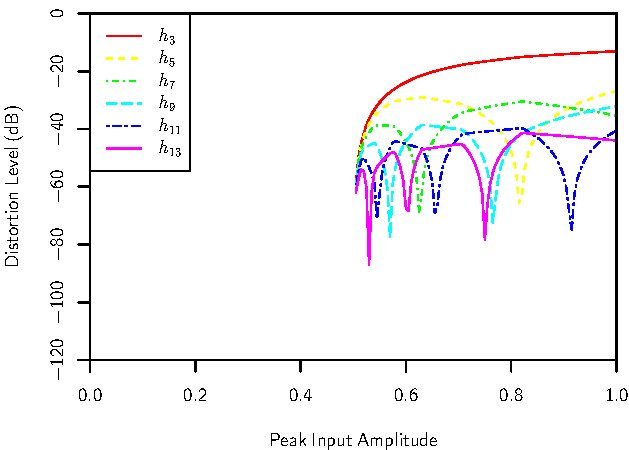
\includegraphics{chapter5/Images/HardClippingHarmonics.pdf}
				\caption{Individual harmonic distortion levels for a symmetric hard peak clipper
					 (Equation~\ref{eq:SymmetricHardClipping}) with a threshold of 0.5.}
				\label{fig:HardClippingHarmonics}
			\end{figure}

			\begin{figure}[h!]
				\centering
				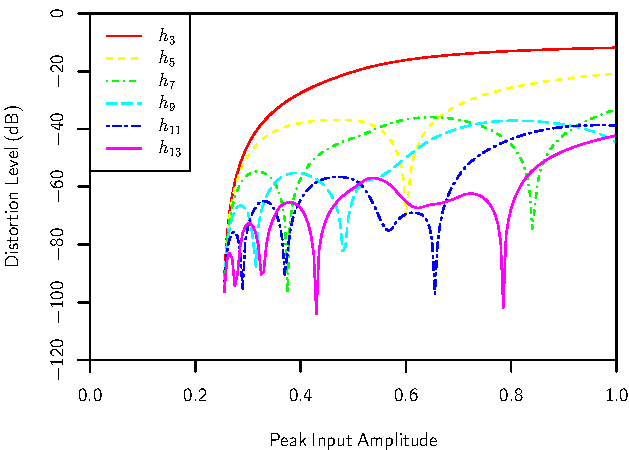
\includegraphics{chapter5/Images/SoftClippingHarmonics.pdf}
				\caption{Individual harmonic distortion levels for a symmetric soft peak clipper
					 (Equation~\ref{eq:SymmetricSoftClipping}) with a threshold of 0.5.}
				\label{fig:SoftClippingHarmonics}
			\end{figure}

			For both hard and soft peak clippers, the levels of harmonics produced depends on the proportion of
			the input signal which is processed nonlinearly. For signals with amplitudes within the linear
			section of a clipper's characteristic curve, no harmonics are produced. This is evidenced by the
			blank sections of Figures \ref{fig:HardClippingHarmonics} and \ref{fig:SoftClippingHarmonics} for
			low input amplitudes. When the input amplitude exceeds the linear section of the characteristic
			curve additional harmonics are created. As the input amplitude increases further, the amplitudes of
			each of these harmonics vary independently of one another. Furthermore, the way in which the
			amplitude of a particular order of harmonic varies is dependent on the characteristic curve of the
			nonlinearity. These characteristics cause clippers to have vastly different perceived effects
			depending on input amplitude. Clipping functions can be defined which give more uniform changes in
			the levels of distortion components with changes in input amplitude.
			Equation~\ref{eq:SymmetricExponentialClipping} describes a novel clipping function, exponential
			clipping, which has this property.
			
			\begin{equation}
				y[n] = \begin{cases}
					t\sgn(x[n]) & \text{if $\abs{x[n]} > t$} \\
					t\sgn(x[n]) \left(1 - \abs{\frac{x[n]}{t} - \sgn(x[n])}^{E} \right) &
						\text{otherwise}
				\end{cases}, \quad t \geq 0 \ \text{and} \ E > 1
				\label{eq:SymmetricExponentialClipping}
			\end{equation}

			Where $E$ is a second parameter defining the exponent of the system. One advantage of this clipper
			is that it has no linear section, meaning that harmonics are generated for input signals of any
			amplitude. Another advantage is that while the system is still non-homogeneous, the levels of the
			generated harmonics vary monotonically with input amplitude as shown in
			Figure~\ref{fig:ExponentialClippingHarmonics}.

			\begin{figure}[h!]
				\centering
				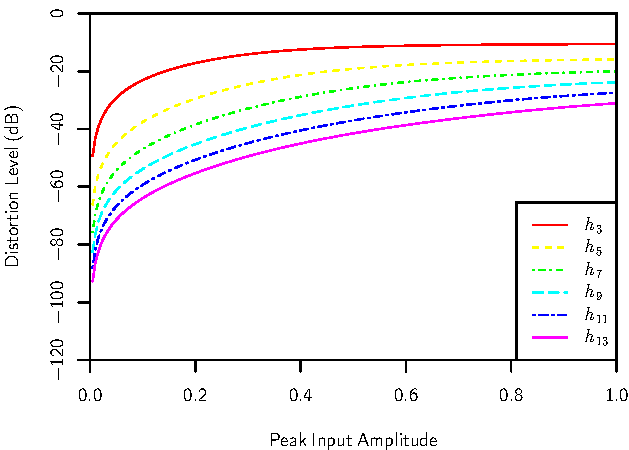
\includegraphics{chapter5/Images/ExponentialClippingHarmonics.pdf}
				\caption{Individual harmonic distortion levels for
					 Equation~\ref{eq:SymmetricExponentialClipping} with a threshold of 0.5 and an 
				         exponent of 5.}
				\label{fig:ExponentialClippingHarmonics}
			\end{figure}

			Simple peak clipping systems can be made homogeneous by introducing gain stages either side of the
			clipping stage as shown in Figure~\ref{fig:HomogeneousClipping}. The first gain stage scales the
			signal such that the clipping stage will always clip the same proportion of the signal. To achieve
			this the amplitude of the input signal must be tracked in order to adjust the gain correctly. The
			second gain stage then scales the signal back to the original input amplitude. In an analogous
			manner the characteristic curve of the clipper can be scaled so it always clips the same proportion
			of the signal, as suggested by \citet{deman2014adaptive}.

			\begin{figure}[h!]
				\centering
				\begin{tikzpicture}
					\node (In) at (0, 1) {$x[n]$};
					\node (InGain) [gain] at (2.5, 1) {};
					\draw (In) -- (InGain);

					\coordinate (MidIn) at (0.75, 1);
					\coordinate (AmpIn) at (0.75, 2);
					\node (Amp) [draw] at (2.5, 2) {Amplitude Follower};
					\draw (MidIn) -- (AmpIn);
					\draw (AmpIn) -- (Amp);
					\draw (Amp) -- (InGain);

					\node (Clip) [draw] at (4.5, 1) {Peak Clipper};
					\draw (InGain) -- (Clip);

					\coordinate (MidOut) at (6.5, 2);
					\node (OutGain) [gain] at (6.5, 1) {};
					\draw (Clip) -- (OutGain);
					\draw (Amp) -- (MidOut) -- (OutGain);

					\node (Out) at (7.5, 1) {$y[n]$};
					\draw (OutGain) -- (Out);
				\end{tikzpicture}
				\caption{Gain stages introduced to make a peak clipping system homogeneous.}
				\label{fig:HomogeneousClipping}
			\end{figure}

		\subsubsection*{Rectification}
			Both half and full wave rectifiers exhibit positive homogeneity. For full wave rectification this
			can be summarised using Equation~\ref{eq:FullWaveRectificationHomogeneity}. For negative values of
			$m$ the right hand side of the equation is the additive inverse of the left hand side. This has
			little effect on the use of a full wave rectifier as the output is always positive.

			\begin{equation}
				\abs{mx[n]} = m\abs{x[n]}, \quad m \geq 0
				\label{eq:FullWaveRectificationHomogeneity}
			\end{equation}

			Half wave rectification behaves slightly differently, in that the sign of the gain applied to a
			signal before processing determines which parts of the signal are zeroed. If a negative gain is
			applied the positive portions of the original input are made negative and are therefore zeroed by
			the rectification. For simple signals, with similar negative and positive portions, this is of no
			concern but for more complex signals the choice of which portions are zeroed may make a perceivable
			difference.

		\subsubsection*{Integrator}
			Integration is a linear operation, meaning that it satisfies the homogeneity principle. The
			implementation given in Equation~\ref{eq:Integrator} however only exhibits positive homogeneity due
			to the rectification of the signal prior to integration. The sign of the gain applied to the input
			signal also determines the points at which the output signal is reset to zero. The signal is reset
			on positive zero crossings but a negative gain applied before the input reverses the direction of
			all zero crossings. Similarly to half wave rectification, this may have audible effects depending
			on the nature of the input signal.

		\subsubsection*{Multiplier}
			Exponentiation is a non-homogeneous operation. Any gain applied to a signal prior to processing is
			also raised to the exponent, as shown in Equation~\ref{eq:MultiplierHomogeneity}.

			\begin{equation}
				(mx[n])^{h} = m^{h}x^{h}[n]
				\label{eq:MultiplierHomogeneity}
			\end{equation}

			As with peak clipping systems, multipliers can be made homogeneous by the addition of a gain stage
			either side of the nonlinearity (as in Figure~\ref{fig:HomogeneousClipping}). For multipliers, this
			effect can only be achieved using gain stages as there is no threshold parameter to change in
			response to the amplitude of the input signal.

		\subsubsection*{\acrshort{ssba}}
			As with multipliers, \acrshort{ssba} is a non-homogeneous process: the gain applied to the input
			signal is raised to the same power as the signal as shown in Equation~\ref{eq:SSBAHomogeneity}.

			\begin{equation}
				\Re \left( (mx_{a}[n])^{h} \right) = m^{h} \Re \left( x_{a}^{h}[n] \right)
				\label{eq:SSBAHomogeneity}
			\end{equation}
			
			Expressing the analytic signal in polar form it can be shown that the amplitude envelope of the
			$h$\super{th} order \acrshort{ssba} is the amplitude envelope of the original signal raised to the
			power $h$, as seen in Equation~\ref{eq:PolarSSBA}.

			\begin{gather}
				x_{a}^{h}[n] = \abs{x_{a}[n]}^{h} e^{ih\arg (x_{a}[n])}
				\label{eq:PolarSSBA}
			\end{gather}

			As the output's amplitude envelope is know in terms of the input's, the output can be normalised in
			an attempt to make the system homogeneous. Multiplying the output of the $h$\super{th} order
			\acrshort{ssba} by $\abs{x_{a}[n]}^{1-h}$ is equivalent to applying $h$\super{th} order
			\acrshort{iap} as shown by Equation~\ref{eq:SSBAandIAP}. The homogeneity of this system is
			discussed in the following section.

			\begin{equation}
				\abs{x_{a}[n]}^{1-h} \Re \left( x_{a}^{h}[n] \right) = 
				\abs{x_{a}[n]} \cos \bigl( h\arg(x_{a}[n]) \bigr)
				\label{eq:SSBAandIAP}
			\end{equation}

		\subsubsection*{\acrshort{iap}}
			The \acrshort{iap} method is homogeneous when used to generate odd order harmonics, but is only
			positive homogeneous when used to generate even order harmonics. Equation~\ref{eq:IAP} is easily
			shown to be positive homogeneous as application of a non-negative gain will alter only the
			amplitude of a signal, leaving its phase information unchanged
			(Equation~\ref{eq:IAPPositiveHomogeneity}).

			\begin{equation}
				\begin{array}{c}
					\abs{mx_{a}[n]} = m\abs{x_{a}[n]} \\
					\arg(mx_{a}[n]) = \arg(x_{a}[n])
				\end{array}
				, \quad m \geq 0
				\label{eq:IAPPositiveHomogeneity}
			\end{equation}

			Application of a negative gain however, changes the phase of the signal
			(Equation~\ref{eq:NegativeGainPhase}).
						
			\begin{equation}
				\arg(mx_{a}[n]) = \bigl( \arg(x_{a}[n]) \bmod 2\pi \bigr) - \pi, \quad m < 0
				\label{eq:NegativeGainPhase}
			\end{equation}

			When the phase is scaled to increase the frequency, the effects depend on the order of the harmonic
			being generated, $h$. The phase of the amplified signal, $mx_{a}[n]$, scaled by $h$ is $h\pi$
			radians less than that of the original signal, $x_{a}[n]$, scaled by the same factor
			(Equation~\ref{eq:IAPOrderHomogeneity}).

			\begin{equation}
				h\arg(mx_{a}[n]) = h \bigl( \arg(x_{a}[n]) \bmod 2\pi \bigr) - h\pi, \quad m < 0
				\label{eq:IAPOrderHomogeneity}
			\end{equation}

			The $-h\pi$ radian offset in phase introduced by the scaling means that the polarity of the output
			is changed depending on the parity of $h$. Odd values of $h$ result in a phase difference of an odd
			multiple of $\pi$ radians, corresponding to an additive inversion of the signal. Even values of $h$
			produce a phase difference of an even multiple of $\pi$ radians, having no effect on the signal. If
			the input signal to a harmonic excitation system using \acrshort{iap} is inverted, the odd order
			harmonics generated will also be inverted while the even order ones will not. This could have
			dramatic timbral effects if the generated harmonics are being summed with other signals that
			include the same frequency components.

		\subsubsection*{Spectral Stretching}
			The phase vocoder algorithm used for spectral stretching is a homogeneous system. When processing
			the signal in the frequency domain only the phase information is altered, leaving the magnitude
			information unchanged. As seen with the analysis of the \acrshort{iap} system, it is possible that
			phase shifts of odd multiples of $\pi$ radians will cause non-homogeneous behaviour. As the phase
			corrections for each new frame of the \acrshort{stft} are calculated iteratively from previous
			frames this should not occur. When processing the first frame the output signal should have the
			same phase information as the input signal avoiding any unwanted signal inversions.

		\subsubsection*{Linear Time Variant Algorithms}
			The remaining algorithms (spectral replication using Equation~\ref{eq:SpectralReplication},
			spectral folding and \acrshort{sttr}) are linear time variant systems. As such they all satisfy the
			principle of homogeneity.

%		\subsubsection*{Spectral Replication}
%			Spectral replication using Equation \ref{eq:SpectralReplication} linear time variant system, as such
%			it satisfies the condition of homogeneity.
%			
%		\subsubsection*{Spectral Folding}
%			Both downsampling and upsampling are homogeneous processes making spectral folding also
%			homogeneous.
%
%			\note
%			{
%				Formal proof?
%			}
%			
%		\subsubsection*{STTR}
%			STTR is a homogeneous process. As the samples in each frame are only multiplied by a constant window
%			and reversed in time none of the amplitude information in the signal is lost. 

	\subsection{Spectral Characteristics}
	\label{sec:ExcitationEvaluation-Comparison-SpectralCharacteristics}
		\subsubsection*{Static Nonlinearities}
			The spectral characteristics of a static nonlinearity depend on the function which describes its
			characteristic curve. If an odd function is used, only odd order distortion components will be
			produced; using an even function, only even order distortion components are generated. A function
			which is neither odd nor even can produce all orders of distortion component. The symmetric
			clippers discussed previously are all described by odd functions. It is evident from the harmonic
			amplitude plots (Figures \ref{fig:HardClippingHarmonics}, \ref{fig:SoftClippingHarmonics} and
			\ref{fig:ExponentialClippingHarmonics}) that only odd order harmonics have been introduced to a
			sinusoidal input. In order to generate even order distortion components these clipping functions
			can be made asymmetric. This is easily done by clipping negative and positive portions of the input
			signal at different thresholds. For example, Equation~\ref{eq:SymmetricHardClipping} can be
			modified to allow for asymmetric clipping giving Equation~\ref{eq:AsymmetricHardClipping}.
			
			\begin{equation}
				y[n] = \begin{cases}
					t_{+} & \text{if $x[n] > t_{+}$} \\
					t_{-} & \text{if $x[n] < t_{-}$} \\
					x[n] & \text{otherwise}
				\end{cases}, \quad t_{-} < t_{+}
				\label{eq:AsymmetricHardClipping}
			\end{equation}

			Where $t_{+}$ and $t_{-}$ are the clipping thresholds for positive and negative portions of the
			signal respectively. Figure~\ref{fig:AsymmetricHardClippingHarmonics} shows the harmonic amplitude
			plot for Equation~\ref{eq:AsymmetricHardClipping} with $t_{+} = 0.5$ and $t_{-} = -0.3$. While the
			system is still non-homogeneous, the introduced energy consists of both odd and even order
			distortion components.

			\begin{figure}[h!]
				\centering
				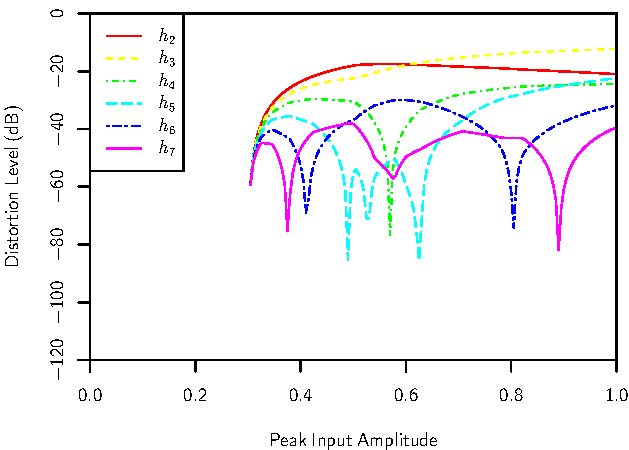
\includegraphics{chapter5/Images/AsymmetricHardClippingHarmonics.pdf}
				\caption{Individual harmonic distortion levels for asymmetric hard clipping
					 (Equation~\ref{eq:AsymmetricHardClipping}) with thresholds of -0.3 and 0.5.}
				\label{fig:AsymmetricHardClippingHarmonics}
			\end{figure}

			For sinusoidal inputs, the amplitudes of the generated harmonics will roll off at differing rates
			depending on the properties of the output signal. The spectrum will roll off at $6(n+1)$dB per
			octave when the $n$\super{th} derivative of the output signal is discontinuous
			\citep{kraght2000aliasing}.  Hard clippers introduce discontinuities to the first derivative of a
			signal and as such will introduce harmonics whose amplitudes will roll off at 12dB per octave.
			Signals clipped by Equation~\ref{eq:SymmetricSoftClipping} are continuous in the first derivative
			and so produce harmonics whose amplitudes roll off at a faster rate. This can be seen in
			Figure~\ref{fig:ClippingSpectra}.

			\begin{figure}[h!]
				\centering
				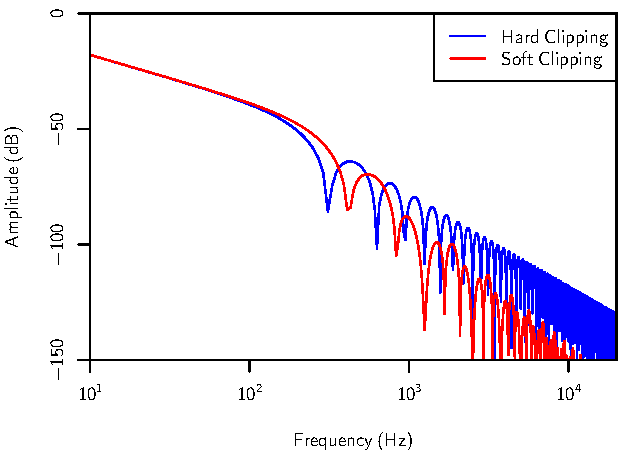
\includegraphics{chapter5/Images/ClippingSpectra.pdf}
				\caption{Spectra of sinusoids clipped using Equations \ref{eq:SymmetricHardClipping} and
			                 \ref{eq:SymmetricSoftClipping}.}
				\label{fig:ClippingSpectra}
			\end{figure}

			The large amount of spectral content introduced by static nonlinearities means they are
			particularly susceptible to aliasing. Through smoothing the characteristic curve of the
			nonlinearity (making the clipper `softer') the amplitudes of generated frequencies will roll off
			more quickly. With lower levels of high order distortion the amplitudes of any aliased components
			will be reduced. Aliasing can also be reduced by creating bandlimited approximations of a static
			nonlinearity's characteristic curve. A simple implementation of this is the harmonic mixer
			\citep{schattschneider1999discrete} in which a low order polynomial expression approximating the
			desired characteristic curve is calculated.  This could be achieved through linear regression as
			shown in Figure~\ref{fig:ClippingApproximation}. The order of the polynomial used controls the
			maximum order of the distortion components generated, effectively eliminating those which would be
			aliased.

			\begin{figure}[h!]
				\centering
				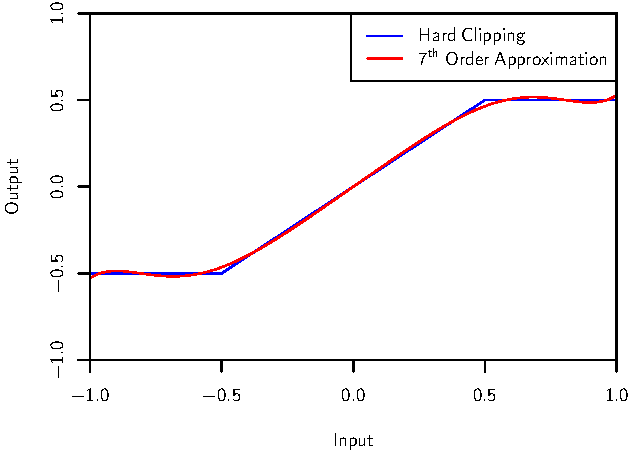
\includegraphics{chapter5/Images/ClippingApproximation.pdf}
				\caption{A 7\super{th} order approximation of hard clipping using linear regression.}
				\label{fig:ClippingApproximation}
			\end{figure}

			Generating characteristic curves in this way reduces the number of aliased frequencies at the cost
			of having to evaluate a more complex polynomial to calculate the output value for each sample. A
			similar approach is used by \citet{fernandez-cid2001distortion} who construct characteristic curves
			from Chebyshev polynomials in order to control the highest frequencies introduced.

			\citet{esqueda2015aliasing} propose a method for the reduction of aliasing in soft clipping
			systems, applying bandlimited hard clipping prior to the soft clipping. They show that their method
			reduced the level of aliased components when processing signals with $f_{0} < 3$kHz. While this
			method does not fully eliminate aliasing, it applies bandlimiting at the Nyquist, ensuring that all
			orders of distortion which will not alias are left mostly unaffected. With a harmonic mixer one
			would have to select a distortion order based on the $f_{0}$ of the input signal to make the best
			use of the bandwidth allowed by the sampling frequency.

		\subsubsection*{Rectification}
			Full wave rectification can be considered as a static nonlinearity with an even characteristic
			curve, as such it only introduces even order distortion components. Examining the Fourier series of
			a full wave rectified sine wave (Equation~\ref{eq:RectificationFourier}) shows the amplitudes of
			each harmonic produced, $c_{n}$ being the amplitude of the $n$\super{th} order harmonic. A full
			derivation of this Fourier series is given in
			Appendix~\ref{app:MathematicalDerivations-Rectification}.

			\begin{gather}
				c_{n} = \frac{1}{2\pi} \int_{-\pi}^{\pi} \abs{sin(x)}e^{-inx} dx \nonumber \\
				c_{n} = \begin{cases}
					\frac{2}{\pi(1 - n^{2})} & \text{when $n$ is even} \\
					0 & \text{when $n$ is odd}
				\end{cases}
				\label{eq:RectificationFourier}
			\end{gather}

			The continuous domain represented by the Fourier series indicates that energy will exist in the
			output at all even order harmonic frequencies. Examining the coefficients, it is apparent that the
			amplitudes of these harmonics roll off at approximately 12dB per octave with no upper bound setting
			the highest frequency generated. In the discrete domain, aliasing will likely occur as there is a
			high probability that significant energy sits at frequencies above the Nyquist.

			The output from a half wave rectifier has the same spectrum as that of a full wave rectifier but
			with the content of the original signal included. This can easily be shown by considering how a
			half wave rectified signal can be constructed from the original signal and a full wave rectified
			signal.  Where $x[n]$, $x_{f}[n]$ and $x_{h}[n]$ represent the original signal, full wave rectified
			and half wave rectified signals respectively, their relationship can be seen in
			Equation~\ref{eq:RectificationRelationship}.

			\begin{equation}
				x_{h}[n] = \frac{1}{2} \left( x_{f}[n] + x[n] \right)
				\label{eq:RectificationRelationship}
			\end{equation}

		\subsubsection*{Integrator}
			Applying the integrator described in Equation~\ref{eq:Integrator} to a sine wave produces a signal
			with Fourier series coefficients as shown in Equation~\ref{eq:IntegratorFourier}. A full derivation
			of this Fourier series is given in Appendix~\ref{app:MathematicalDerivations-Integrator}.

			\begin{gather}
				c_{n} = \frac{kf_{s}}{2\pi} \left( \int_{0}^{\pi} \bigl( 1 - cos(x) \bigr) e^{-inx} dx +
							\int_{\pi}^{2\pi} \bigl( 3 + cos(x) \bigr) 
							e^{-inx} dx \right) \nonumber \\
				c_{-1} = - \frac{2ikf_{s}}{\pi} \nonumber \\
				c_{0} = 2kf_{s} \nonumber \\
				c_{1} = \frac{2ikf_{s}}{\pi} \nonumber \\
				c_{n} = \frac{ikf_{s}}{\pi} \left( \frac{2n^{2} + e^{-in\pi} - 1}{n^{3} - n} \right)
				\label{eq:IntegratorFourier}
			\end{gather}

			This produces all harmonics with amplitudes rolling off at approximately 6dB per octave. This
			shallow roll off makes integrators very useful when a large amount of new frequency content is
			desired. Due to the shallow roll off of the distortion components' amplitudes, integrators are very
			prone to aliasing. While integrators are homogeneous, they are frequency dependent, exhibiting low
			pass filter characteristics. Using the same integration constant, a high frequency input signal
			will produce a lower amplitude output than a low frequency input. This does not affect the
			relative amplitudes of frequencies in the output, just the overall amplitude of the signal.

		\subsubsection*{Multiplier}
			Nonlinear processing using a multiplier (Equation~\ref{eq:Multiplier}) in which the exponent is a
			positive integer, allows for control over the maximum order of distortion generated. The highest
			frequency present among those generated will be equal to the highest frequency in the input signal
			multiplied by the exponent, $h$. This effect is illustrated by applying a multiplier to an
			arbitrary compound signal. This signal has an $f_{0}$ of 1kHz and has energy in its first four
			harmonics, making the highest frequency present 4kHz. Its spectrum is shown in
			Figure~\ref{fig:FourHarmonics}.

			\begin{figure}[h!]
				\centering
				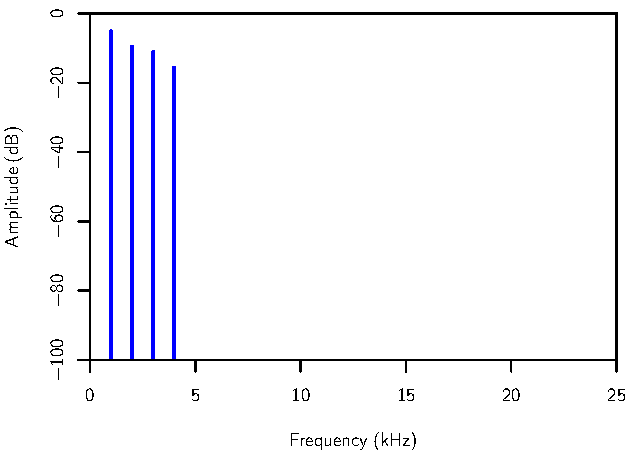
\includegraphics{chapter5/Images/FourHarmonics.pdf}
				\caption{The spectrum of the signal used to illustrate the spectral characteristics of
					several algorithms.}
				\label{fig:FourHarmonics}
			\end{figure}
			
			Figure~\ref{fig:CubedSpectra} shows the spectral effects of cubing the signal shown in
			Figure~\ref{fig:FourHarmonics}. After cubing the signal, the highest frequency is three times that
			in the input signal, moving from 4kHz to 12kHz. This upper bound on the order of distortion
			introduced allows for effective reduction / elimination of aliasing. As the highest frequency in
			the output is $h$ times that in the input, ensuring the input has no frequency components over
			$\frac{f_{s}}{2h}$Hz ensures that all frequency components in the output will be below the Nyquist.
			Low pass filtering the input at this frequency is an effective means of reducing the aliasing
			introduced.

			\begin{figure}[h!]
				\centering
				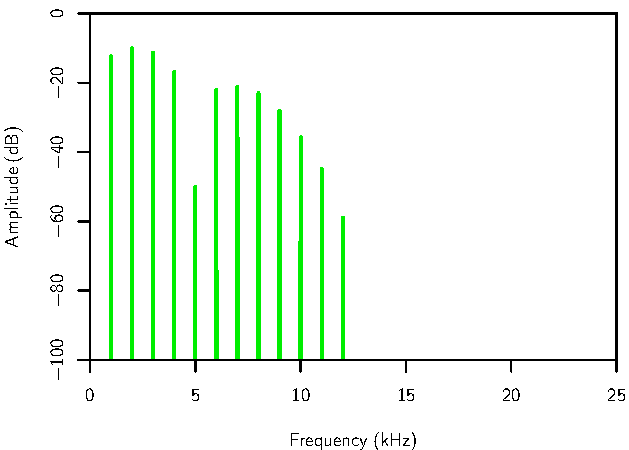
\includegraphics{chapter5/Images/CubedSpectra.pdf}
				\caption{The spectral effects of cubing the signal represented in
					Figure~\ref{fig:FourHarmonics}.}
				\label{fig:CubedSpectra}
			\end{figure}

			For an exponential static nonlinearity (one in which the exponent can take any positive value)
			control over the bandwidth of the output signal is lost. Non-integer exponents cause higher orders
			of distortion to be generated. Figure~\ref{fig:TwoAndAHalfSpectra} shows the spectral effects of
			raising the same input signal to the power 2.5. Here it is evident that there is no upper bound on
			the order of distortion components generated. The lowest frequency component in the output signal
			is not bound regardless of the exponent used.  For even exponents the output will always be
			positive, meaning there will always be some 0Hz (DC offset) energy introduced.

			\begin{figure}[h!]
				\centering
				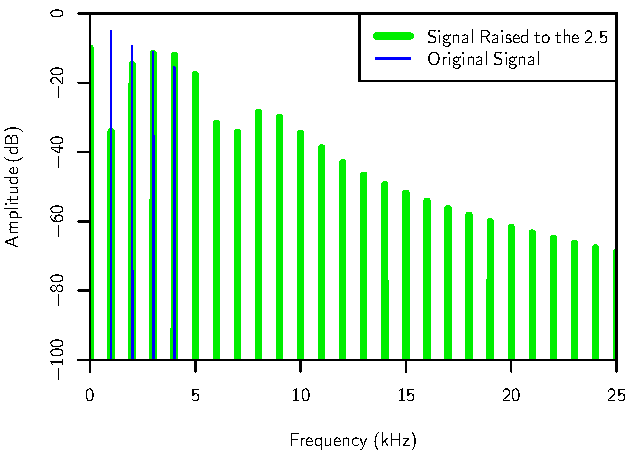
\includegraphics{chapter5/Images/RaisedToTwoAndAHalfSpectra.pdf}
				\caption{The spectral effects of raising the signal represented in
					Figure~\ref{fig:FourHarmonics} to the power 2.5.}
				\label{fig:TwoAndAHalfSpectra}
			\end{figure}

		\subsubsection*{\acrshort{ssba}}
			\acrshort{ssba} extends the control provided by multipliers as it constrains the minimum frequency
			introduced as well as the maximum. Using Equation~\ref{eq:SSB}, only the upper sideband (the sum
			frequencies) of the modulation is produced. The highest and lowest frequency components of the
			output are those of the input signal multiplied by the exponent, $h$. All other harmonic and
			intermodulation components created lie between these two frequencies. This can be seen in
			Figure~\ref{fig:SSBA3Spectra}, which shows the results of applying $3$\super{rd} order
			\acrshort{ssba} to the signal shown in Figure~\ref{fig:FourHarmonics}.
			
			\begin{figure}[h!]
				\centering
				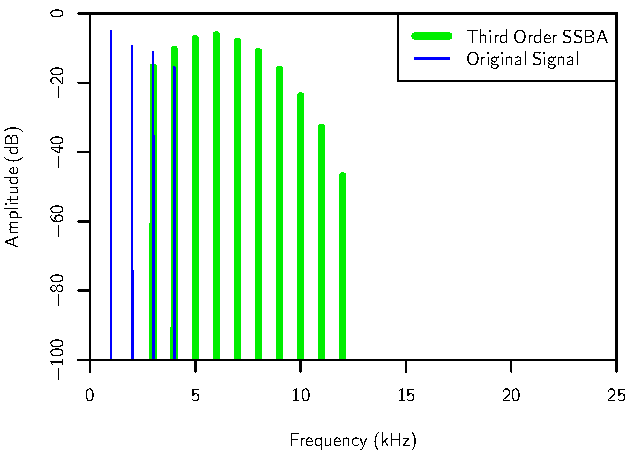
\includegraphics{chapter5/Images/SSBA3Spectra.pdf}
				\caption{The spectral effects of applying third order \acrshort{ssba} to the signal
					represented in Figure~\ref{fig:FourHarmonics}.}
				\label{fig:SSBA3Spectra}
			\end{figure}

			As with a multiplier, the bound \acrshort{ssba} gives on the maximum frequency in the output allows
			for effective control of aliasing. Again, low pass filtering the input at $\frac{fs}{2h}$Hz prior
			to processing will remove those components in the input that will be aliased when processed.

			This bounding of the frequencies in the output signal means that \acrshort{ssba} will produce a
			single harmonic if the input is a sinusoid, as shown in Equation~\ref{eq:OneSideband}. This is
			useful in situations in which fine control is required over the content of the output spectrum. An
			output signal can be constructed through the generation of several individual harmonics.

		\subsubsection*{\acrshort{iap}}
			Like the \acrshort{ssba} method, if the input is sinusoidal the \acrshort{iap} method will generate
			a single harmonic. In contrast to the \acrshort{ssba} method, the \acrshort{iap} method provides
			little control over the bandwidth of the output when the input has multiple frequency components.
			Figure~\ref{fig:IAP3Spectra} shows the spectral effects of third order \acrshort{iap} processing on
			the same signal shown in Figure~\ref{fig:FourHarmonics}.

			\begin{figure}[h!]
				\centering
				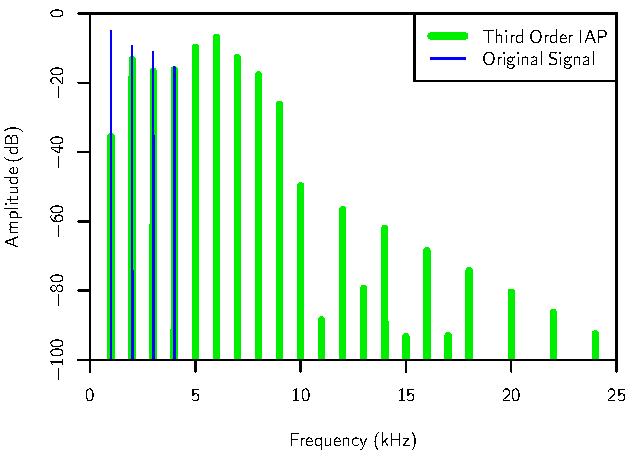
\includegraphics{chapter5/Images/IAP3Spectra.pdf}
				\caption{The spectral effects of applying third order \acrshort{iap} to the signal
				represented in Figure~\ref{fig:FourHarmonics}.}
				\label{fig:IAP3Spectra}
			\end{figure}

			When multiple frequency components are present in the input signal, \acrshort{iap} processing
			produces energy at high order distortion components. The exact orders and amplitudes of the
			distortion components produced are dependent on the content of the input signal and the order of
			\acrshort{iap} applied. As with previous algorithms, it may be necessary to upsample the signal
			before processing to avoid aliasing of these frequencies.

		\subsubsection*{Spectral Replication}
			In spectral replication each frequency component is shifted by the same amount, preserving the
			differences between them. This is useful for harmonic excitation of simple harmonically structured
			signals; providing the spectrum is shifted by an integer multiple of the $f_{0}$, any components at
			harmonic frequencies in the input will remain harmonic frequencies at the output. Being an
			\acrshort{ltv} system, spectral replication avoids the intermodulation distortion inherent to the
			systems discussed previously. 

			Due to every frequency component being shifted by an equal amount, the bandwidth of the output is
			equal to that of the input. This predictability allows for easier control of the output spectrum.
			It also provides a simple method for the reduction of aliasing: the highest frequency in the output
			will be that of the input plus the shift frequency $f$. Applying a low pass filter, with a cutoff
			frequency of $\left( \frac{f_{s}}{2} - f \right)$Hz to the input signal will minimise the amplitude
			of any aliased frequency components.

		\subsubsection*{Spectral Folding}
			Spectral folding with a factor $k$ results in the lowest $\frac{1}{k}$ of the input spectrum being
			repeated $k$ times in the output spectrum. Every second repetition being a mirror image of the
			original, as shown previously in Figure~\ref{fig:SpectralFolding}. The new frequencies introduced
			in the output depend on the sampling rate of the signal. Unless $\frac{f_{s}}{2k}$ is a harmonic of
			the input signal, there is little chance that the new frequencies will be harmonically related to
			the input. Other than changing the downsampling / upsampling factor $k$, the user is given little
			control over the content of the output spectrum.  The bandwidth of the output is not constricted,
			possibly taking up the entirety of the spectrum.  Additional filtering is needed to shape the
			output spectrum as desired, increasing the overall complexity of the system.

		\subsubsection*{Spectral Stretching}
			An ideal spectral stretching system would produce the result shown in
			Figure~\ref{fig:SpectralStretching}. All frequency components are scaled by the same factor
			preserving the frequency ratios between spectral components. For harmonically structured signals
			this has the effect of scaling the $f_{0}$, increasing the signal's perceived pitch. For a
			sinusoidal input this results in the generation of individual harmonics as with the \acrshort{ssba}
			and \acrshort{iap} techniques.
			
			The phase vocoder introduces frequency artefacts during its operation. The process of splitting the
			signal into frames causes spectral leakage; energy at a given frequency is spread across the nearby
			frequencies. This can cause inharmonic partials to be generated for input signals which are
			perfectly harmonic. To counteract this, a window function can be applied to the frames prior to
			calculating their \acrshort{dft}. Various different window functions have been proposed, each
			having different effects in reducing the spectral leakage. The selection of a window function is
			application specific, the performance and use of several different functions is discussed by
			\citet{harris1978on}.
			
			Ignoring the effects of spectral leakage, the bandwidth of the output signal will be that of the
			input multiplied by the stretching factor. This allows for effective minimisation of aliasing as
			the signal can be low pass filtered prior to processing as done with multipliers and
			\acrshort{ssba}.
		
		\subsubsection*{\acrshort{sttr}}
			The spectral effects of \acrshort{sttr} depend on the properties of the input signal and the
			window function and step size used. For simple sinusoidal inputs, complex output spectra can be
			generated. For example, consider the spectral effects of \acrshort{sttr} using the window function
			defined in Equation~\ref{eq:STTRWindow} (shown in Figure~\ref{fig:STTRWindow}). This window
			function exhibits constant overlap add for a step size of $\frac{L}{2}$.
			Figure~\ref{fig:STTRSpectra} shows the output spectra of \acrshort{sttr}, using this window with
			lengths of 1ms and 1.5ms, on a 1kHz sinusoid.

			\begin{equation}
				w[n] = \begin{cases}
					\cos \left( \frac{4\pi n}{3L} \right) & \text{if $\abs{n} \leq \frac{L}{4} $} \\
					1 - \cos \left( 2\pi \frac{2n - \sgn(n)L}{3L} \right) &
						\text{if $\frac{L}{4} < \abs{n} \leq \frac{L}{2}$} \\
					0 & \text{otherwise}
				\end{cases}
				\label{eq:STTRWindow}
			\end{equation}

			\begin{figure}[h!]
				\centering
				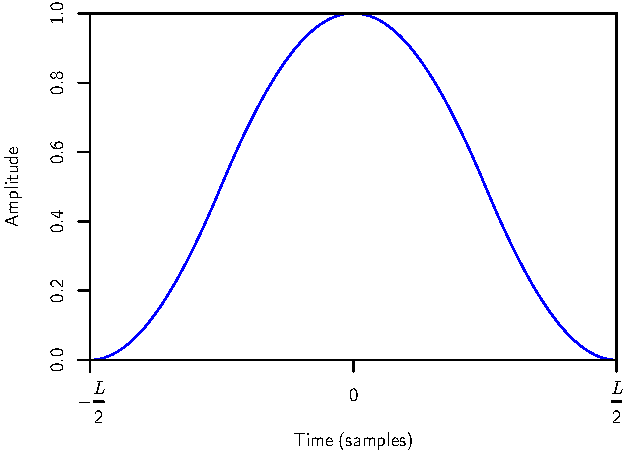
\includegraphics{chapter5/Images/STTRWindow.pdf}
				\caption{The window function defined in Equation~\ref{eq:STTRWindow}.}
				\label{fig:STTRWindow}
			\end{figure}

			\begin{figure}[h!]
				\centering
				\captionsetup[subfigure]{oneside,margin={1cm, 0cm}}
				\subfloat[1ms Window]
				{
					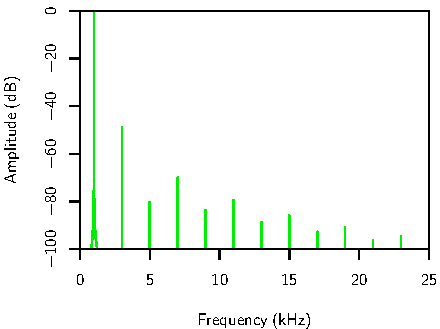
\includegraphics{chapter5/Images/STTRSpectra1.pdf}
					\label{fig:STTR1ms}
				}
				\quad
				\subfloat[1.5ms Window]
				{
					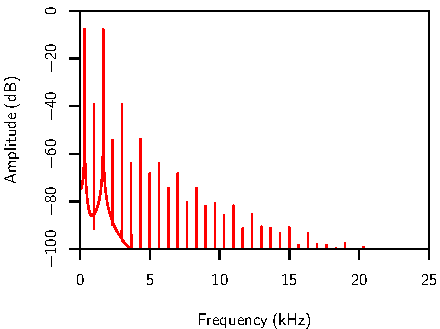
\includegraphics{chapter5/Images/STTRSpectra1p5.pdf}
					\label{fig:STTR1p5ms}
				}
				\caption{The spectral effects of applying \acrshort{sttr} to a 1kHz sinusoid using
					different window lengths.}
				\label{fig:STTRSpectra}
			\end{figure}

			The period of the output signal is equal to the least common multiple of the input signal's period
			and the step size. If the period of the input signal is an integer multiple of the step size this
			means the period will remain unchanged by the processing. This is evidenced by the output spectrum
			produced by use of a 1ms window, shown in Figure~\ref{fig:STTRSpectra}. Only odd order harmonics
			are generated retaining the original period of the signal. When a signal's period is not an integer
			multiple of the step size it is increased by \acrshort{sttr}. The output spectrum for a 1.5ms
			window shows this, the period of the signal being increased to 3ms. The lowest frequency in this
			output is then approximately 333Hz.

			The exact frequencies of the partials in the output are discussed by \citet{kim2014shorttime}. In
			effect they are the intermodulation frequencies of the input frequency and the step frequency. The
			amplitudes of these partials are influenced by the Fourier transform of the window function used.
			This allows the spectral characteristics of the output to be loosely controlled through
			manipulation of the window function and step size. There is no upper bound on the frequency of the
			output so upsampling may need to be used to minimise aliasing.

	\subsection{Temporal Characteristics}
	\label{sec:ExcitationEvaluation-Comparison-TemporalCharacteristics}
		\subsubsection*{Static Nonlinearities}
			As static nonlinearities are memoryless (i.e. non of the previous input and output samples are
			needed for the calculation of the current output sample) they can not easily be used to control the
			temporal evolution of a signal. The gradient of the characteristic curve for low amplitude samples
			can be manipulated to alter the attack and release times of signals. Increasing the gradient will
			shorten attack and release times, while decreasing it will lengthen them. As an extreme example
			consider the infinite peak clipper shown in Equation~\ref{eq:InfinitePeakClipper}.

			\begin{equation}
				y[n] = \sgn(x[n])
				\label{eq:InfinitePeakClipper}
			\end{equation}
			
			Figure~\ref{fig:InfinitePeakClipping} shows a signal, with attack and release sections, before and
			after infinite peak clipping. The original signal rises to its full amplitude over two cycles and
			falls back to silence over the same time. After infinite peak clipping, the attack and release have
			become instantaneous.

			\begin{figure}[h!]
				\centering
				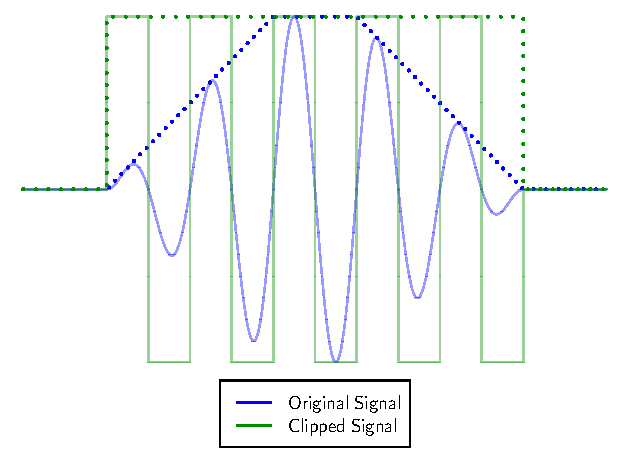
\includegraphics{chapter5/Images/InfinitePeakClipping.pdf}
				\caption{The amplitude envelopes of a signal before and after infinite peak clipping.}
				\label{fig:InfinitePeakClipping}
			\end{figure}

			The exact change in attack / release time is dependent on both the characteristic curve of the
			nonlinearity and the existing temporal features of the input signal. For the infinite peak clipper,
			all dynamic information in a signal is lost and all attack and release times are made
			instantaneous. Other static nonlinearities, such as soft peak clippers, have less predictable
			effects on temporal envelopes. 

		\subsubsection*{Rectification}
			Full wave rectifiers have no effect on the temporal characteristics of signals as the magnitude
			information of each sample is preserved, however it is possible that a half wave rectifier could
			change the position of the onset / offset of a signal by a small amount. If a signal starts with a
			negative displacement, the first section of the signal would be removed, moving the onset to the
			position at which the first positive displacement occurs. This possible delay in onset however, is
			highly dependent on the input signal and will most likely be imperceptible.
			
		\subsubsection*{Integrator}
			Due to the inherent low pass filtering behaviour of integrators (see
			Section~\ref{sec:ExcitationEvaluation-Comparison-SpectralCharacteristics}) the temporal properties
			of transient signals will be altered. Fast rise times will be lengthened by the attenuation of
			their high frequency components as seen in Figure~\ref{fig:IntegratorTemporalEffects}. This
			prevents integrators being used for harmonic excitation in applications where it is essential that
			transients are preserved. 

			\begin{figure}[h!]
				\centering
				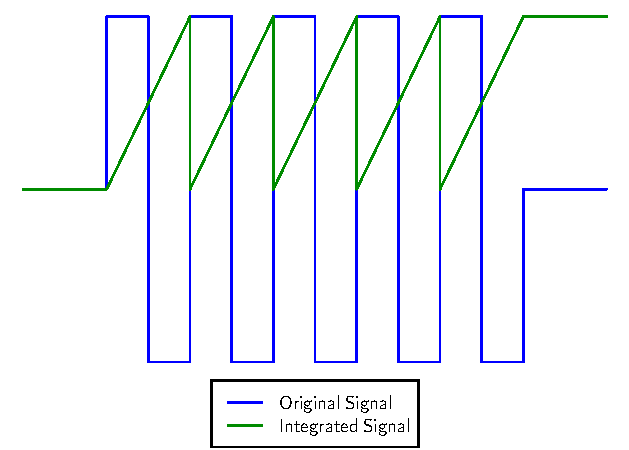
\includegraphics{chapter5/Images/IntegratorTemporalEffects.pdf}
				\caption{The effects of an integrator on the rise time of a signal.}
				\label{fig:IntegratorTemporalEffects}
			\end{figure}
			
		\subsubsection*{Multiplier}
			Multipliers and exponential static nonlinearities have a dynamic compression / expansion effect.
			For exponents greater than one the dynamics of a signal are expanded, the amplitude difference
			between low and high amplitude portions of the signal is increased. For exponents less that one the
			opposite occurs, compressing the dynamics of the signal. Figures
			\ref{fig:MultiplierTemporalEffects} and \ref{fig:ExponentiationTemporalEffects} show the effects
			this can have on the attack and release portions of signals.

			\begin{figure}[h!]
				\centering
				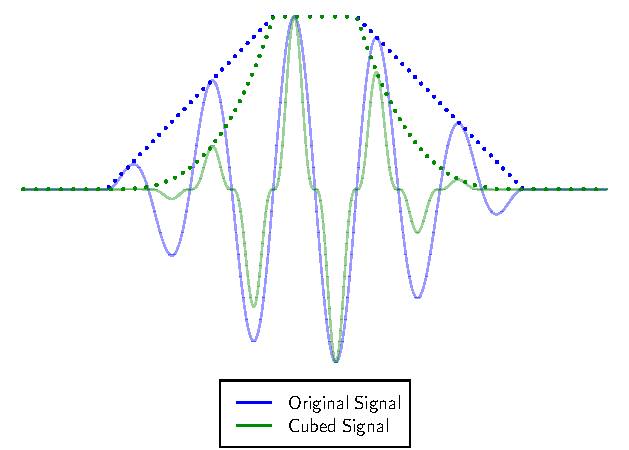
\includegraphics{chapter5/Images/MultiplierTemporalEffects.pdf}
				\caption{The amplitude envelopes of a signal before and after cubing.}
				\label{fig:MultiplierTemporalEffects}
			\end{figure}

			\begin{figure}[h!]
				\centering
				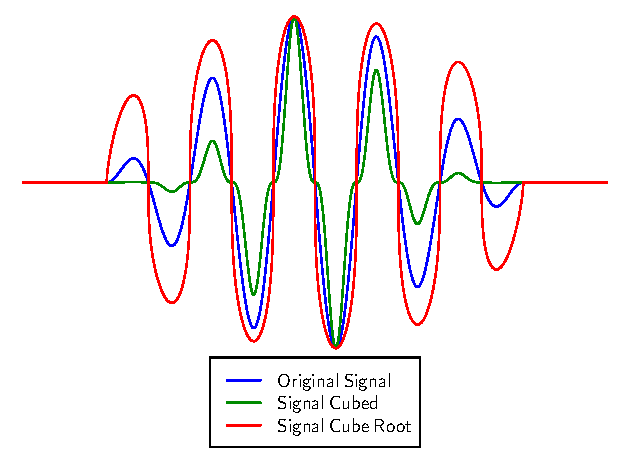
\includegraphics{chapter5/Images/ExponentiationTemporalEffects.pdf}
				\caption{The amplitude envelopes of a signal before and after cube rooting.}
				\label{fig:ExponentiationTemporalEffects}
			\end{figure}

			While the time taken for the signal to rise to or decay from maximum amplitude is not changed, the
			shape of the amplitude envelope during the attack and release portions is. Exponents greater than
			one cause the amplitude to rise more slowly initially and then rapidly rise, while exponents less
			than one increase the initial gradient of the attack and then slowly rise to full amplitude. As
			with other static nonlinearities these effects are dependent on the input signal and are not
			predictable enough to give intuitive control.

		\subsubsection*{\acrshort{ssba}}
			\acrshort{ssba} has similar temporal effects to a multiplier. The signal undergoes dynamic
			expansion, changing the shape of its attack and release envelopes as shown in
			Figure~\ref{fig:SSBATemporalEffects}.  The restricted bandwidth of the \acrshort{ssba} technique's
			output is also apparent from this graph. The input is a sinusoid with a simple amplitude envelope.
			The output is a sinusoid with three times the frequency and an amplitude envelope equal to that of
			the input cubed. This is in contrast to the effect of the multiplier shown in
			Figure~\ref{fig:MultiplierTemporalEffects} where the output signal is no longer sinusoidal.

			\begin{figure}[h!]
				\centering
				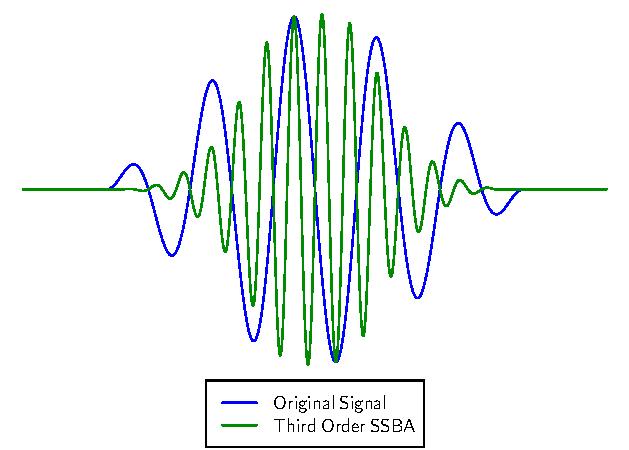
\includegraphics{chapter5/Images/SSBATemporalEffects.pdf}
				\caption{The amplitude envelopes of a signal before and after 3\super{rd} order
					 \acrshort{ssba}.}
				\label{fig:SSBATemporalEffects}
			\end{figure}

		\subsubsection*{\acrshort{iap}}
			\acrshort{iap} alters only the frequency (phase) information of a signal. As the amplitude
			information is left unaltered, the system preserves the input signal's amplitude envelope. Due to
			this the temporal characteristics of signals are unaffected. This can be seen in
			Figure~\ref{fig:IAPTemporalEffects} where it is apparent that the frequency of the sinusoid has
			been altered and its amplitude envelope not.

			\begin{figure}[h!]
				\centering
				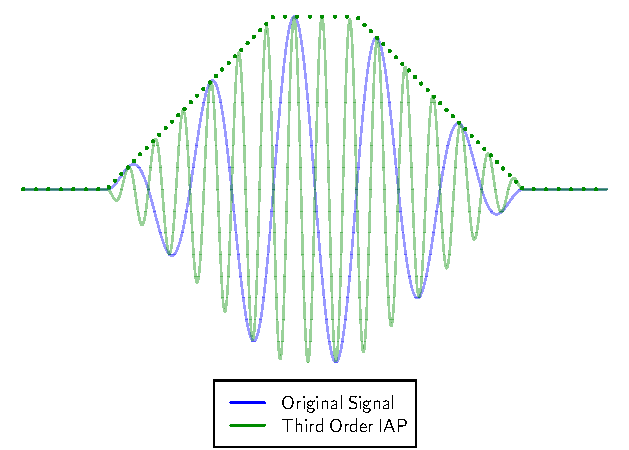
\includegraphics{chapter5/Images/IAPTemporalEffects.pdf}
				\caption{The amplitude envelopes of a signal before and after 3\super{rd} order
					 \acrshort{iap}.}
				\label{fig:IAPTemporalEffects}
			\end{figure}
			
		\subsubsection*{Spectral Replication}
			Spectral replication using Equation~\ref{eq:SpectralReplication} operates by multiplying the
			analytic signal by a unity amplitude complex sinusoid. This has the effect of multiplying a
			signal's amplitude envelope by one, leaving it unaffected.
			Figure~\ref{fig:SpectralReplicationTemporalEffects} illustrates this, showing the effects on a
			signal's amplitude envelope by shifting it's frequency content upwards by 1.5Hz

			\begin{figure}[h!]
				\centering
				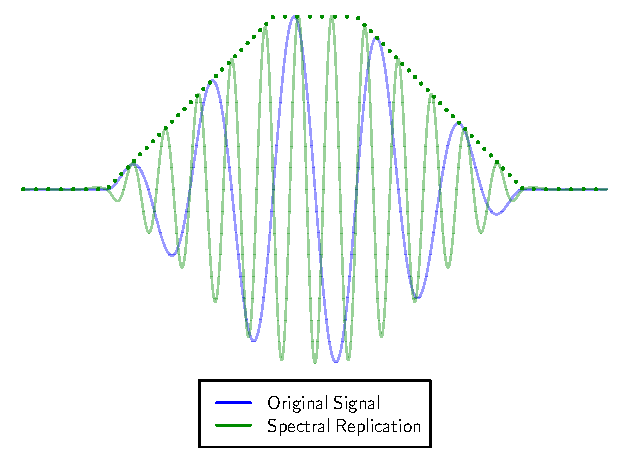
\includegraphics{chapter5/Images/SpectralReplicationTemporalEffects.pdf}
				\caption{The amplitude envelopes of a signal before and after spectral replication.}
				\label{fig:SpectralReplicationTemporalEffects}
			\end{figure}

		\subsubsection*{Spectral Folding}
			When using spectral folding, the low pass filter applied prior to the downsampling and upsampling
			process removes the high frequency content which contributes to transients in the signal. This has
			the effect of lengthening attack times similar to the effect seen in the integrator system. The
			degree, $k$, of spectral folding determines the cutoff frequency of the filter; higher values of
			$k$ removing more high frequency energy, causing longer attack times.

		\subsubsection*{Spectral Stretching}
			A simple phase vocoder implementation produces artefacts when processing transients in a signal.
			The phase correction stage before resynthesis can have the effect of softening the attack portion.
			The exact effect had on the transient is not able to be controlled as it depends on where the
			transient lies in the \acrshort{stft} frame. \citet{robel2003a} proposes a method to better process
			transients with a phase vocoder. First, an algorithm is used to detect the presence of transients
			in an \acrshort{stft} frame, the phase information is then processed differently depending on the
			position of the transient within the frame.

		\subsubsection*{\acrshort{sttr}}
			Due to the time reversal, \acrshort{sttr} can have complicated effects on a signal's amplitude
			envelope.  For instance, the attack and release portion of a sound may be switched. Whilst
			possible, this is highly dependent on the window length, step size and spectral content of the
			input signal. Controlling these aspects for general input signals proves a very difficult task.

	\subsection{Use Cases}
	\label{sec:ExcitationEvaluation-Comparison-UseCases}
		\subsubsection*{Static Nonlinearities}
			Static nonlinearities prove useful for situations in which a large band of new spectral energy
			needs to be created efficiently and the precise spectral structure is not important. For musical
			signals, static nonlinearities introduce a spectrally dense band of audio, the spectral content of
			which is highly dependent on that of the input signal. Properties of the characteristic curve can
			be changed in order to control the orders of distortion components in the output as well as the
			rate at which their amplitudes roll off. Further shaping of the spectrum is most easily applied
			through additional filtering. Typical static nonlinearities, such as peak clippers, are
			non-homogeneous, although steps can be taken to improve on this at the cost of introducing
			additional complexity.
			
		\subsubsection*{Rectification}
			Rectifiers find use in the same applications as other static nonlinearities but due to the
			properties of the characteristic curve, their effects are better defined. In rectification, only
			even order distortion components are generated, for sinusoidal inputs this amounts to a series of
			even harmonics with amplitudes reducing by 12dB per octave. Rectifiers may be more useful for
			timbral control than other static nonlinearities due to their exhibiting positive homogeneity.

		\subsubsection*{Integrator}
			Integrators are similarly useful to general static nonlinearities, they provide an efficient means
			to add wideband energy to the spectrum of a signal. The implementation discussed in this work
			(Equation~\ref{eq:Integrator}) has similar properties to a rectifier, being a positive homogeneous
			system which introduces distortion components with a shallow roll off. The primary difference being
			that the integrator produces all orders of distortion rather than only even orders. A disadvantage
			of integrators over rectifiers is that they smear transients due to their low pass filtering
			effect.

		\subsubsection*{Multiplier}
			Multipliers offer greater spectral flexibility than peak clippers, rectifiers and integrators,
			giving control over the orders of distortion introduced. This allows for better control of the
			bandwidth of the output signal, placing a bound on the maximum frequency in the output. A harmonic
			mixer (described in Section~\ref{sec:ExcitationEvaluation-Comparison-SpectralCharacteristics}) can
			be constructed in which the output of several multipliers with different exponents can be summed in
			order to include multiple orders of distortion. This increases the control over the output spectrum
			at the expense of increasing the computational complexity. In use cases where aliasing distortion
			needs to be eliminated, a harmonic mixer can be used to approximate the behaviour of other static
			nonlinearities.

		\subsubsection*{\acrshort{ssba}}
			\acrshort{ssba} increases the flexibility of a multiplier further. As only the sum sideband of the
			intermodulation is generated, the minimum frequency in the output signal is bounded as well as the
			maximum. When the input is sinusoidal the output will be an individual harmonic. Building a
			harmonic mixer using \acrshort{ssba} provides full control over which harmonics are generated from
			a sinusoidal input. Where fine control of the spectral output is desired, \acrshort{ssba} provides
			a reasonably low complexity solution. One disadvantage of this method is its non-homogeneous
			behaviour which could be amended using similar techniques as those used for peak clippers
			(discussed in Section~\ref{sec:ExcitationEvaluation-Comparison-Homogeneity}).

		\subsubsection*{\acrshort{iap}}
			\acrshort{iap} can be used in similar ways to \acrshort{ssba}. For sinusoidal inputs the output is
			an individual harmonic, meaning harmonic mixers can be constructed which provide very fine spectral
			control. \acrshort{iap} is possibly more applicable in this situation than \acrshort{ssba} as it a
			homogeneous / positive homogeneous system, depending on the order of distortion being applied. Care
			may need to be taken if mixing odd and even orders of distortion as the behaviour of the system is
			slightly different for each. This homogeneity is gained at the expense of less predictable
			behaviour when used to process signals with more than one frequency component compared to
			\acrshort{ssba}. If the input signal is more complex than a sinusoid it may be preferential to use
			\acrshort{ssba}.

		\subsubsection*{Spectral Replication}
			Spectral replication provides a way of generating higher order harmonics without unwanted
			intermodulation components being introduced. To ensure that the harmonic structure is preserved,
			the $f_{0}$ of the input signal must be accurately tracked in order to determine how much the
			frequency should be shifted by. A discussion of different $f_{0}$ tracking methods is given in
			Section~\ref{sec:FeatureControl-Systems-Fundamental}. While this introduces considerable
			complexity, the bandwidth of the output is bounded at both ends and the system is homogeneous. The
			spectral envelope of the output is the same as that of the input, so further filtering is required
			to apply any other manipulations.

		\subsubsection*{Spectral Folding}
			Spectral folding is an efficient method of producing energy throughout the output spectrum.
			However, it does not provide sufficient control to ensure that the new spectral partials are
			harmonically related to those in the input. The effects are highly dependent on the content of the
			input signal as well as the sampling frequency.

		\subsubsection*{Spectral Stretching}
			Spectral stretching is similar to \acrshort{ssba} in that it imposes a bound on the maximum and
			minimum frequencies in the output. A perfect spectral stretching system would produce only harmonic
			distortion components, having an advantage over \acrshort{ssba} in which intermodulation must be
			combated. In practice, using a phase vocoder, artefacts are introduced and the complexity of the
			system exceeds that of \acrshort{ssba} considerably.

		\subsubsection*{\acrshort{sttr}}
			\acrshort{sttr} can be used, much like a static nonlinearity, as a method of generating wide bands
			of high order harmonics. Unlike static nonlinearities however, it is possible to generate
			inharmonic partials for a sinusoidal input. The generation of these partials is dependent on the
			properties of the input signal, adding further complexity to predicting the effects for arbitrary
			input signals.  \citet{kim2015harmonizing} suggest methods through which the output of
			\acrshort{sttr} can be controlled for use as a harmonising effect. This effect introduces new tones
			at specific musical intervals depending on the input frequency. While this is useful as a creative
			tool for music composition, it does not provide the uniform response across input signals required
			for timbral control.

\section{Conclusion}
	This chapter has discussed the characteristics of the harmonic generation algorithms presented in
	Chapter~\ref{chap:Excitation}, highlighting their desirable / undesirable traits when applied to timbral control.
	A full summary of the findings for each algorithm was shown in Table~\ref{tab:ComparisonSummary}. In brief, two
	broad classes of harmonic generators are identified; those which generate large numbers of distortion components
	with little control over their frequencies / amplitudes and those which provide control over the orders of
	distortion introduced, sometimes allowing for the generation of individual harmonics. There is typically a
	compromise made between control and computational complexity; algorithms providing more control over the resulting
	spectrum requiring more computation.

	Static nonlinearities and integrators are the best choice where a large series of distortion components need to be
	created efficiently. The traditionally used peak clipper might not be the most suitable for intuitive timbral
	control due to its non-homogeneity. Rectifiers and integrators however, are both positive homogeneous systems.
	Selecting between rectification and integration depends on the characteristics required for a timbral manipulation.
	Rectification will only generate even order distortion components but will have negligible effects on any temporal
	properties of a signal. Integration generates all orders of distortion but has a low pass filter response which
	will increase the attack times of input transients. Neither of these methods provide any control over the maximum
	order of distortion introduced, leading to possible problems with aliasing. Bandlimited rectification can be
	applied by modelling its characteristic curve with a harmonic mixer. As integration is not a static nonlinearity it
	cannot be bandlimited in this manner.

	Where finer control over the spectral structure of the output is desired, more complex algorithms are needed. Here
	\acrshort{ssba}, \acrshort{iap} and spectral stretching have desirable characteristics. Each of these algorithms
	are able to generate individual harmonics from a sinusoidal input and each have their own advantages and
	disadvantages. Spectral stretching is the most computationally intensive of the three and the phase vocoder
	approach is prone to the introduction of artefacts. \acrshort{ssba} and \acrshort{iap} are both simpler systems and
	each has a particular advantage. For purely sinusoidal input, \acrshort{iap} outperforms \acrshort{ssba} in that it
	is positive homogeneous, having no effect on the amplitude envelope of a signal. For more complex inputs however,
	\acrshort{ssba} may be preferential as it provides more control over the range of frequencies in the output,
	bounding the orders of intermodulation components generated. In
	Section~\ref{sec:PerceptualExperiments-Reconstruction} perceptual listening tests are carried out in order to
	evaluate the perceived quality of individual harmonics generated using both \acrshort{ssba} and \acrshort{iap}.

	In Chapter~\ref{chap:FeatureControl} the analysis of harmonic generation algorithms discussed in this chapter is
	used to inform the design of harmonic excitation systems. The properties of the algorithms identified allow these
	systems to be configured to control specific audio features (defined in Chapter~\ref{chap:Timbre}) of an input
	signal.
